\documentclass[11pt,twoside,letterpaper,onecolumn,english]{article}
\bibliographystyle{h-physrev5}


% LATEX PACKAGES
\usepackage[english]{babel}                  % ?
\usepackage{graphicx}                            % graphics
\usepackage{amsfonts,amsmath,amssymb}  % math symbols
\usepackage[switch]{lineno}                   % line numbers for draft
\usepackage[small,compact]{titlesec}   % to squeeze the doc a bit
\usepackage{mathptmx}                          % switch font default to times
\usepackage[square,numbers,sort&compress]{natbib}   % short numerical refs
\usepackage{hyperref}                             % links in PDF
\usepackage{xcolor}                                 % colored text (for comments)
\usepackage{listings}                               % code font
\usepackage{xspace}                               % spaces after commands
\usepackage{ragged2e}


% MARGINS AND SPACING
\usepackage[left=1in,top=1in,right=1in,bottom=1in,nohead]{geometry}

%\setlength{\parskip}{0in}
%\setlength{\parindent}{1em}
%\setlength{\parsep}{0pt}
%\setlength{\headsep}{0pt}
%\setlength{\topskip}{0pt}
%\setlength{\topmargin}{0pt}
%\setlength{\topsep}{0pt}
%\setlength{\partopsep}{0pt}
%\setlength{\bibsep}{0.0pt}


%\documentclass[modern]{desc-tex/styles/lsstdescnote}

% LATEX PACKAGES
%\usepackage{desc-tex/styles/lsstdesc_macros}

\usepackage{xcolor}
\usepackage{authblk}

\begin{document}
\markboth{Photometric Redshift Data Challenge}{Photometric Redshift Data Challenge}

\title{Photometric Redshift Data Challenge}
\author[1,2]{Eric Charles}
\author[3]{Qianjun Hang}
\author[4]{Josue De Santiago}
\author[5]{Leonel Media-Varela}
\author[6]{Justin Myles}
\author[7]{Samuel J.  Schmidt}
\author[8,9]{Tianqing Zhang}
\affil[1]{\small SLAC National Accelerator Laboratory, 2575 Sand Hill Road, Menlo Park, CA 94025, USA}
\affil[2]{Kavli Institute for Particle Astrophysics and Cosmology (KIPAC), Stanford University, Stanford, CA 94305, USA}
\affil[3]{Department of Physics \& Astronomy, University College London, Gower Street, London WC1E 6BT, UK}
\affil[4]{Secihti---Departamento de F\'isica, Centro de Investigaci\'on y de Estudios Avanzados del I.P.N. Apdo. 14-740, Ciudad de M\'exico 07000, M\'exico}
\affil[5]{McWilliams Center for Cosmology and Astrophysics, Department of Physics, Carnegie Mellon University, Pittsburgh, PA, USA}
\affil[6]{Department of Astrophysical Sciences, Princeton University, Princeton, NJ 08544, USA}
\affil[7]{Department of Physics and Astronomy, University of California, One Shields Avenue, Davis, CA 95616, USA}
\affil[8]{Department of Physics and Astronomy and PITT PACC, University of Pittsburgh, Pittsburgh, PA 15260, USA}
\affil[9]{LSST Interdisciplinary Network for Collaboration and Computing Frameworks, 933 N. Cherry Avenue, Tucson AZ 85721, USA}
\date{\today}

\maketitle

\begin{abstract}
  Many Rubin science cases will require photometric redshift (PZ)
  estimation. We are organizing a PZ data challenge to assess the
  current status of PZ algorithms and analysis pipelines. This
  document describes the format of the PZ challenge, including the
  data that participants will use, the tasks that they will
  be asked to perform, and the metrics and criteria by which submissions will
  be assessed. It also provides detailed instructions for how to
  submit entries to the challenge.  
\end{abstract}


\section{Introduction}
\label{sec:intro}

Redshift inference is a key element of many DESC science
goals, and redshift uncertainty is one of the leading contributors to
overall uncertainty on cosmological models from imaging survey
data.  Precursor surveys took a variety of approaches to this problem,
accounting for differences in underlying data as well as modeling
approaches.  In all cases, redshift uncertainty was significantly
larger than the DESC Science Requirements listed in the LSST DESC Science
Requirements Document.

This state of the art motivates a data challenge to characterize and
improve existing methods, as well as to provide infrastructure for the
development of improved methods. Overall, this requires generating
uniform input catalogs to use and infrastructure for comparing output
redshift posteriors to each other and to simulated truth catalogs.


\section{Photometric redshift basics}
\label{sec:redshift_basics}

Photometric redshift estimation involves taking a catalog of galaxies
for which we have observations in several different filters and have
measured the brightness of the galaxies in those bands, and
using that information to estimate the redshift of the galaxies.
For LSST we expect to have measurements in 6 bands: 'u', 'g', 'r',
'i', 'z', and 'y', covering a wavelength range from approximately 
320 to 1600 nanometers. For the Roman space telescope, this will
extend from about 500 to 2300 nanometers.

Much of the information used to estimate photometric redshifts derives
from the 'Balmer break' present in the rest frame of many spectra at
400 nm. As the break crosses into different optical filters with
increasing redshift, the differences in magnitudes between filters
carry information about the redshift; see, e.g.,
Fig.~\ref{fig:pz_redshift_basics}. This can also be seen when
plotting redshifts as a function of derived colors, i.e., differences
in magnitudes between filters; see, e.g., Fig.~\ref{fig:color_color_redshift}.

\begin{figure*}[ht]
  \centerline{
    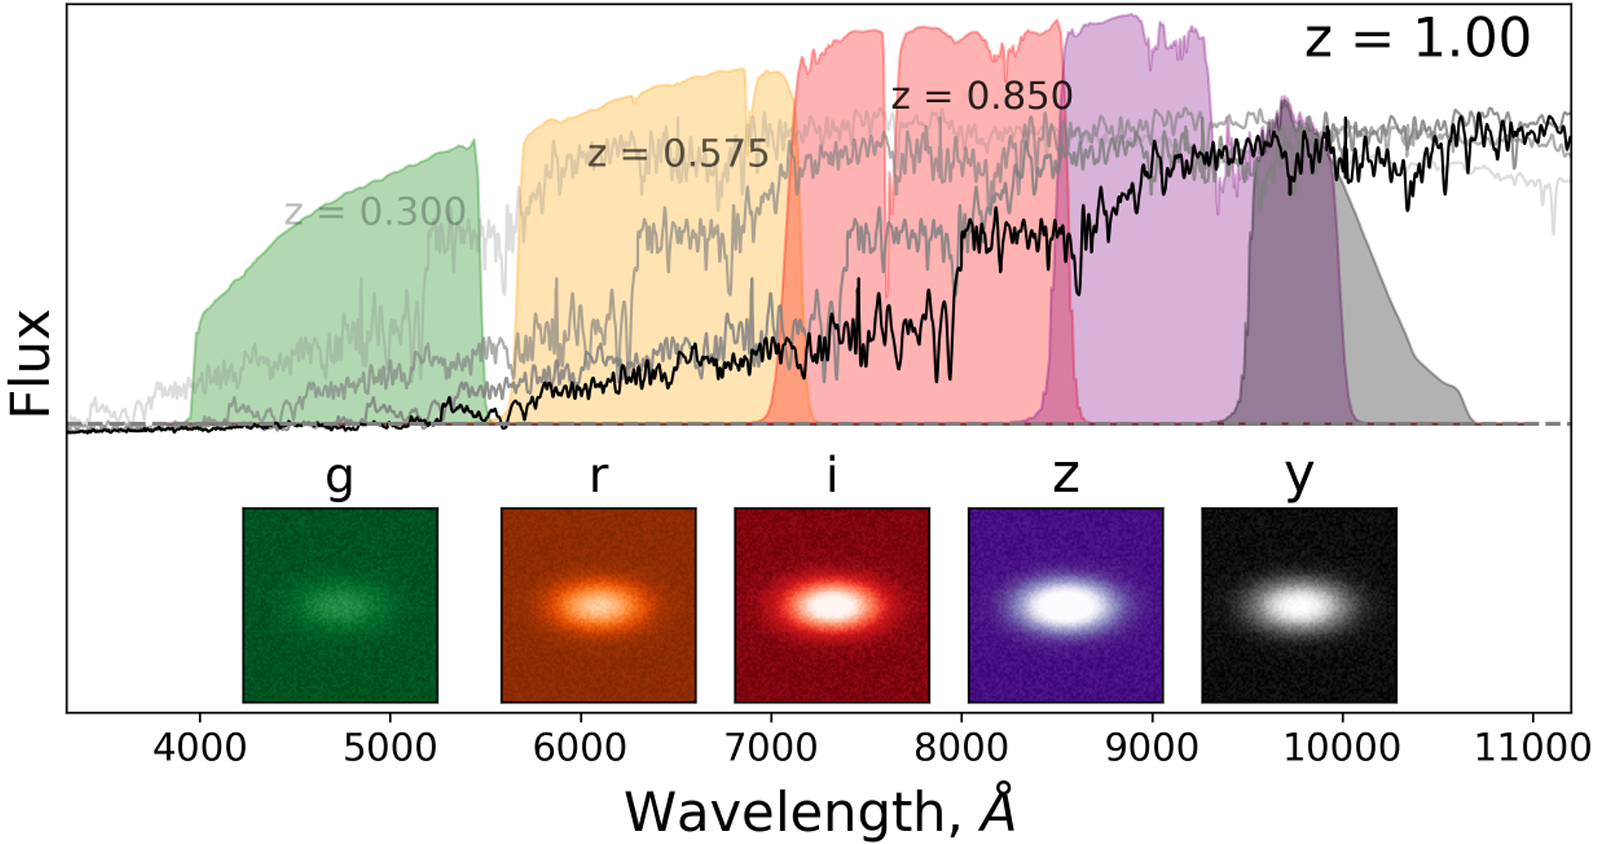
\includegraphics[width=0.80\textwidth]{figures/static_balmer.png}    
  }
  \caption{\label{fig:pz_redshift_basics}\small{A passive galaxy at
      different redshifts and how it will show up in various optical
      filters, giving us the ability to estimate its redshift and
      therefore distance. For many galaxies, the so-called
      'Balmer break' at 400 nm is a reliable feature that causes the
      flux to drop severely in bluer filters. Figure and caption
      by Jamie McCullough.}}
\end{figure*}

\begin{figure*}[ht]
  \centerline{
    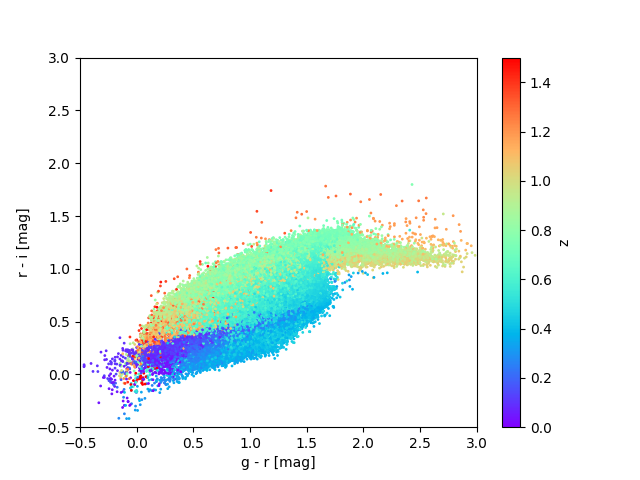
\includegraphics[width=0.45\textwidth]{figures/color_color_redshift_taskset_1_cardinal_10yr}    
    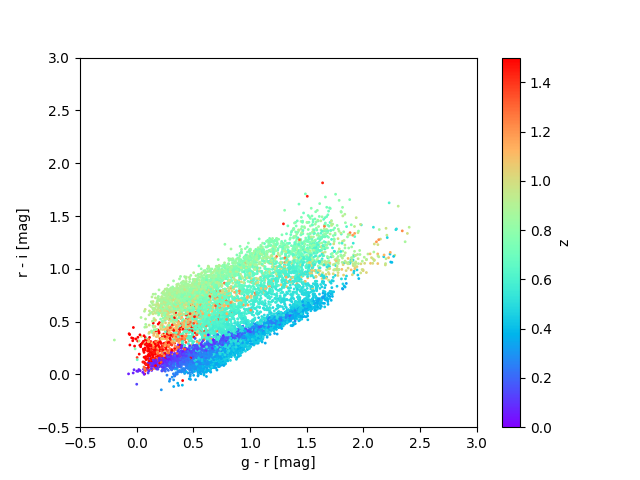
\includegraphics[width=0.45\textwidth]{figures/color_color_redshift_taskset_1_flagship_10yr}
  }
  \caption{\label{fig:color_color_redshift}\small{Redshifts plotted as
      a function of $r-i$ versus $g-r$ colors for a sample of objects
      in the cardinal (left) and flagship (right) simulations. These
      are plotted for the data for task set 1, i.e., for a sample of
      objects with $i < 23$.}}
\end{figure*}

This overly simple picture is complicated somewhat by the fact that
different galaxies have different intrinsic spectra and colors, as
seen in Fig.~\ref{fig:color_redshift}.

\begin{figure*}[ht]
  \centerline{
    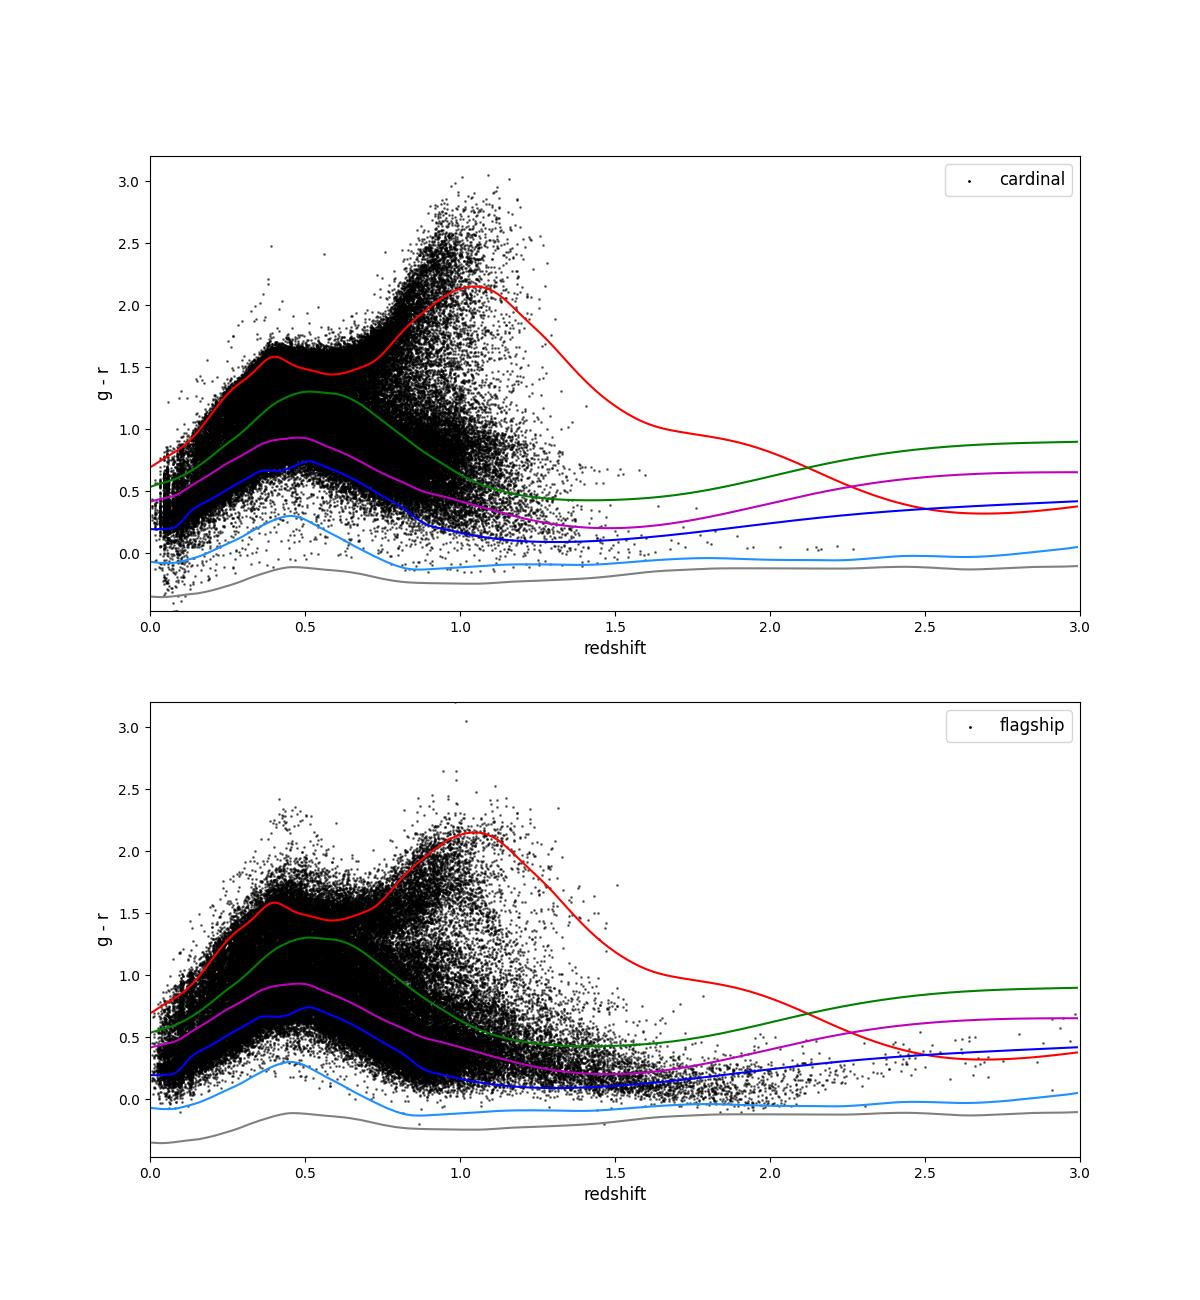
\includegraphics[width=0.80\textwidth]{figures/gr_vs_sz_sidebyside.jpg}    
  }
  \caption{\label{fig:color_redshift}\small{Color ($g-r$) plotted as a function of
      redshift for a sample of objects in the cardinal (top) and
      flagship (bottom) simulations. These are plotted for the data
      for task set 1, i.e., for a sample of objects with $i < 23$. The
      overlaid lines show the templates for several different types of galaxies.}}
\end{figure*}

This is further complicated by the fact that reference redshifts,
typically obtained by spectroscopy, slitless spectroscopy (i.e., GRISM
measurements), or narrowband photometric measurements, are not a
representative sample, as they are much easier to obtain for brighter
objects. Depending on the method used to obtain the reference
redshifts, they are also susceptible to errors such as confusing
different spectral lines or confusion of blended objects. Some of
the tasks in this data challenge encourage participants to try to
address these complications.


\section{Challenge Format}
\label{sec:challenge_format}

The PZ data challenge comprises a series of sets of tasks for participants.
Submissions will be evaluated to determine how ready various algorithms are
to be used for cutting-edge analysis based on how well they perform on
the various tasks. Readiness will be evaluated on a few different
fronts: 1) Does the algorithm meet performance requirements? 2) Is
it robust, flexible, and relatively easy to use on different datasets?
3) Is it scalable up to the scales we will need to use it at?

This document and the associated web pages describe the data being
provided to participants, the tasks they will be asked to perform, the
expected format for submission and the metrics by which the algorithm
readiness will be evaluated.


\subsection{Scope and Timeline}

The data challenge will include two major parts, with a set of
tasks emulating increasingly realistic scenarios in each part. The
first part, $p(z)$ estimation, will focus on estimating the redshift of
individual objects. The second part, tomography and $n(z)$ estimation,
will focus on assigning objects to tomographic bins and estimating the
distribution of redshifts in each bin.

The data challenge will run from April 13, 2026 to August 7, 2026.
The first set of data and tasks related to $p(z)$ estimation will be
released on April 13. A second set of data and tasks related to more
realistic $p(z)$ estimation scenarios and $n(z)$ estimation will be
released on June 1.

Preliminary results will be released on August 14, 2026, with a
technical note summarizing those results to follow shortly thereafter and
a comprehensive journal publication to follow later.


\subsection{Installing and setting up the \texttt{pz\_data\_challenge}
  package}

The \texttt{pz\_data\_challenge} package will provide participants with tools
to access data, set up submissions, estimate performance metrics and
format submissions.  This can be set up with a few small
variants on the standard \texttt{GitHub} package setup procedure.
Before starting you should pick a name for your submission, e.g., ``example''.

\begin{verbatim}
# Create a conda environment
conda create --name pzdc python=3.13

# Clone the pz_data_challenge repository (or your fork of the repository)
git clone git@github.com:LSSTDESC/pz_data_challenge.git
# or git clone https://github.com/LSSTDESC/pz_data_challenge.git

# Go into the directory
cd pz_data_challenge

# Install the code in "editable" mode
pip install -e ".[dev]"

# Use the provided script to set up your submission.
# Here you should provide the name of your submission
python scripts/prepare_submission.py <submission_name>
\end{verbatim}

This final step will copy the input data files to
\texttt{pz\_data\_challenge/public}, and set up the three files you will
need to submit your entry.

The notebooks in the \texttt{pz\_data\_challenge/nb} area give examples
of how to access the data and create some of the diagnostic plots
that were used to validate the data.


\subsection{Submission mechanism}

Submission will take the form of pull request in the
\texttt{pz\_data\_challenge} repository.  Detailed instructions on how
to submit an entry are provided in
Sec.~\ref{sec:challenge_submissions} of this document.


\section{Challenge Input Data}
\label{sec:challenge_input_data}

The preparation of the challenge data is described in the appendices.
The data are available as a \texttt{tar} archive that is downloaded and
unpacked as part of the \texttt{pz\_data\_challenge} setup procedure.

Each task set in the data challenge has an associated set of files.
Typically these will be a collection of training files that contain
photometric data and reference redshifts, and a second set of files
that contain photometric data but do not include redshifts. Each
task set will involve estimating something about the redshifts or
redshift distributions in the test files.

Typically there will be several training and test files for a
particular task set, covering different scenarios and using different
input simulations.


\subsection{Input data format}

The input data for the challenge are presented in HDF5 files.
The naming convention for the files is
\texttt{\{challenge\}\_\{taskset\}\_\{simulation\}\_\{label\}\_\{scenario\}.hdf5}.
The meanings of the various \allowbreak fields are described in
Tab.~\ref{tab:file_fields}. The columns in the files are described
in Tab.~\ref{tab:columns}.  We note that we use \texttt{np.nan} to in
the magnitude columns to signify non-detections.

\begin{table}[ht]
\centering
\caption{\label{tab:file_fields}\small Fields in the input file names.}
\begin{tabular}{ll}
  \hline\hline  
  Field & Description \\ \hline
  challenge & Challenge associated with file (``pz\_challenge'') \\
  taskset & Task set associated with file (e.g., ``taskset\_1'') \\
  simulation & Simulation used to produce file (``cardinal'' or ``flagship'') \\
  label & File label (e.g., ``test'', ``training'') \\
  scenario & Data scenario (e.g., ``1yr'', ``10yr'') \\
\hline\hline
\end{tabular}
\end{table}


\begin{table}[ht]
\centering
\caption{\label{tab:columns}\small Contents of input files.}
\begin{tabular}{ll}
  \hline\hline
  Column & Description \\ \hline  
  redshift & True redshift (training files only) \\
  ra & Right ascension (training files only) \\
  dec & Declination (training files only) \\
  object\_id & Unique object ID\\
  mag\_\{band\}\_lsst & Magnitude in LSST \{band\} \\
  mag\_\{band\}\_lsst\_err & Magnitude uncertainty in LSST \{band\} \\
  mag\_\{band\}\_roman & Magnitude in Roman \{band\} \\
  mag\_\{band\}\_roman\_err & Magnitude uncertainty in Roman \{band\} \\
\hline\hline
\end{tabular}
\end{table}

We note that the \texttt{table-io} package~
\cite{tables_io} installed with
\texttt{pz\_data\_challenge} provided a command line interface to
convert files from \texttt{hdf5} format to other formats such as
\texttt{parquet} tables or \texttt{pandas} data frames.

\begin{verbatim}
# convert a hdf5 file to pandas dataframe in a parquet file
tables-io convert
  --input public/pz_challenge_taskset_1_cardinal_test_10yr.hdf5
  --output public/pz_challenge_taskset_1_cardinal_test_10yr.pq
\end{verbatim}


\section{Challenge Submissions}
\label{sec:challenge_submissions}

\subsection{Challenge subtask types}

The challenge is organized as a series of sets of tasks using
increasingly realistic representations of the data. In general, each
set of tasks includes 3 subtasks.

\begin{enumerate}
  \item{Estimate either per-object $p(z)$ or ensemble $n(z)$
      distributions for a set of different scenarios and provide the
      estimates in a specified format.}
  \item{Provide trained models for the different scenarios and a
      Python function that can be used to generate the estimates from subtask
      1 on an arbitrary dataset.}    
  \item{Provide a Python function that can be used to
      generate the models and estimates from subtasks 1 and 2 on
      arbitrary datasets.}
\end{enumerate}

The $p(z)$ estimates in subtask 1 and the trained models in subtask 2 should be provided
in a compressed \texttt{tar} file, which is described below.   Templates and instructions for the
Python functions needed for subtasks 2 and 3 will be provided and are
described below.


\subsection{\texorpdfstring{Data format for per-object $p(z)$ estimates}{Data format for per-object p(z) estimates}}

The $p(z)$ estimates should be submitted in \texttt{qp} format,
which allows users to specify a complete $p(z)$ distribution for
each object, as well as summary statistics for each object.

The \texttt{qp} package~\cite{QP} supports several different representations of
$p(z)$, such as different functional forms as well as interpolated
grids, histograms, and others.

For users unfamiliar with \texttt{qp}, we highly recommend representing
the $p(z)$ as either an interpolated grid or a Gaussian mixture model.

\begin{verbatim}
# Interpolated grid
import qp
import numpy as np
# Define the x-grid. Note that we put all the
# p(z) on the same x-grid
xvals = np.array([0,0.5,1,1.5,2])
# Define the y-values. Note we provide n_grid_points x n_objects 
# values, as we need to provide a y-value at each grid point 
# for each object.
yvals = np.array(
 [
   [0.01,0.2,0.3,0.2,0.01],
   [0.1,0.3,0.5,0.2,0.05]
 ]
)
ensemble = qp.interp.create_ensemble(xvals,yvals)
ensemble.write_to(<output_filename.hdf5>)
\end{verbatim}

\begin{verbatim}
# Mixture model
import qp
import numpy as np
# Define the means, standard deviations, and weights.
# These should each have shape n_objects, n_components.
# In this case we are defining 3 objects with 2-Gaussian 
# representations.
# For each object the weights should sum to 1, or they
# will be normalized.
means = [[0.3, 0.4], [0.5, 0.5], [0.6, 0.8]]
stds = [[0.2, 0.4], [0.1, 0.3], [0.05, 0.3]]
weights = [[0.8, 0.2], [0.7, 0.3], [0.8, 0.2]]
ensemble = qp.mixmod.create_ensemble(means=means,stds=stds,weights=weights)
ensemble.write_to(<output_filename.hdf5>)
\end{verbatim}

The submission files should use the same file name conventions defined
in Tab.~\ref{tab:file_fields}. The labels will typically be
\texttt{pz\_estimate} or \texttt{pz\_model} and will be specified in
the descriptions of the various tasks, e.g.,

\begin{verbatim}
\texttt{pz\_challenge\_taskset\_1\_cardinal\-\_pz\_estimate\_1yr.hdf5}
  or
\texttt{pz\_challenge\_taskset\_1\_cardinal\_pz\_model\_1yr.pkl}.
\end{verbatim}

All of these files should then be joined into a \texttt{tar} file, which 
should then be placed somewhere it can be download.  The URL for the
\texttt{tar} should be specified in
\texttt{tests/test\_\{submission\}.py}

\begin{verbatim}
SUBMISSION_NAME = "example"
SUBMISSION_URL = "https://your.institution.edu/submit_example.tgz"
\end{verbatim}


\subsection{Format for estimation-only Python functions and trained models}

For the second subtask, submissions should provide trained models and
implement a function to run estimation using those trained models on
the test files provided for each task set. The function will look something like this:

\begin{verbatim}
def run_taskset_1_estimation_only(
    model_file: str | Path,
    test_file: str | Path,
    output_file: str | Path,
) -> None:
    # do stuff and write p(z) estimates to "output_file"
\end{verbatim}

or

\begin{verbatim}
def run_taskset_2_estimation_only(
    model_file: str | Path,
    test_file: str | Path,
    output_file: str | Path,
) -> None:
    # do stuff and write p(z) estimates to "output_file"
\end{verbatim}

Templates for these functions are provided in the file
\texttt{tests/test\_\{submission\}.py} created as part of the setup.


\subsection{Format for training and estimation Python functions}

For the third subtask, submissions should implement a function to
train models and run estimation using those trained models on the
training and test files provided for each task set. The function will
look something like this:

\begin{verbatim}
def run_taskset_1_training_and_estimation(
    train_file: str | Path,
    test_file: str | Path,
    output_file: str | Path,
) -> None:
    # train a model using the "train_file" and make p(z) estimates 
    # and write them to "output_file"
\end{verbatim}

or

\begin{verbatim}
def run_taskset_2_training_and_estimation(
    train_file: str | Path,
    test_file: str | Path,
    output_file: str | Path,
) -> None:
    # train a model using the "train_file" and make p(z) estimates
    # and write them to "output_file"
\end{verbatim}

Templates for these functions are provided in the file
\texttt{tests/test\_\{submission\}.py} created as part of the setup.


\subsection{Submission mechanism}

Submissions will take the form of a pull request on the
\texttt{pz\_data\_challenge} repository and will include:

\begin{enumerate}
  \item{A file \texttt{tests/test\_\{submission\}.py} that includes the
      URL from which the compressed \texttt{tar} file should be downloaded
      as well as the Python functions for subtasks 2 and 3.   When
      created this will contain empty placeholder functions that will
      need to be implemented.}
   \item{A file \texttt{requirements\_\{submission\}.txt} that should
       be modified to include \texttt{pip} package names of any
       packages that need to be installed in order to run the
       functions in subtasks 2 and 3.}     
   \item{A file \texttt{.github/workflows/submit\_\{submission\}.yaml} to
       run the submission validation in a GitHub action.  This should
       not need to be modified unless the prerequisites installation
       requires more than just \texttt{pip}  installing packages.}
\end{enumerate}

All three of these files are created by the
\texttt{scripts/prepare\_submission.py} script.  

You will need modify the \texttt{tests/test\_\{submission\}.py} to
give the location of the \texttt{tar} file containing the PZ estimates
and trained models, and to implement the require functions.

See \texttt{https://github.com/LSSTDESC/pz\_data\_challenge/pull/6}
for an example of a submission.


\subsection{Submission validation}

The wrapping functions provided in the \texttt{tests/test\_\{submission\}.py}
file implement a number of \allowbreak checks on the data. Specifically, for each
expected file they check that:

\begin{enumerate}
    \item{the file exists;}
    \item{the file contains a valid \texttt{qp} ensemble;}
    \item{the \texttt{qp} ensemble includes ancillary data;}
    \item{the ancillary data includes a 'zmode' column with redshift
        estimates;}
    \item{the ancillary data includes an 'object\_id' column;}
    \item{the object\_ids in the submission file match the associated
        test file.}
\end{enumerate}

If any of these checks fail, the GitHub action triggered by the
submission will fail and report the cause of the failure.  \textbf{Note that
the github actions occasionally fail to download the data files.  If this happens
simply rerunning the action typically succeeds.}

The easiest way to test that you have correctly implemented the
required functions is simply to run these commands.

\begin{verbatim}
# Make sure that you have installed any packages you need
pip install -r requirement_{submission_name}.txt

# Run the functions you have provided as unit tests
py.test tests/test_{submission_name}.py
\end{verbatim}

if this succeeds, you can use a provided script to help you open the
pull request for your submission.

\begin{verbatim}
# run the submission helper script.
python scripts/submit.py {submission_name}
\end{verbatim}

Note that the help script only prints the required commands, it does
not run them.  In short the command are:

\begin{verbatim}
# Check status of your local git clone by running git status, and make
# sure that you are on the branch submit/{submission_name} and do not
# have any files added or modified
git status

# Add your files to git
git add .github/workflows/submit_example.yaml
  requirements_example.txt
  tests/test_example.py

# Commit your files to your branch: 
git commit -m "Submitting {submission_name}"
  .github/workflows/submit_{submission_name}.yaml
  requirements_{submission_name}.txt
  tests/test_{submission_name}.py

# Push your commit
git push --set-upstream origin submit/{submission_name}

# Pushing to git should give you a URL that you can visit to create a
# pull request, for example:
#   https://github.com/LSSTDESC/pz_data_challenge/pull/new/submit/example
# Visit that URL and create a pull request, then add the 'submission'
# label to the PR.
# Finally, make sure that the github action validating your submission
# succeeds and fix any issues.
\end{verbatim}


\subsection{Submission aids}

A few scripts are provided to help you.

\begin{itemize}
  \item{\texttt{scripts/download\_public.py}:  downloads and unpacks
      the public data.}    
  \item{\texttt{scripts/prepare\_submission.py}:  sets up your area for
      a submission, creates the needed files from templates and
      downloads the public data, and suggests that you create a branch
      for you submission.}
  \item{\texttt{scripts/remove\_submission\_files.py}:  removes the
      submission files if you need to start over.}
  \item{\texttt{scripts/run\_metrics.py}:  run perfomance metrics on
      files in a submission you have created.}    
  \item{\texttt{py.test tests/test\_\{submission\_name\}.py}:  validates
      all the parts of your submission, checking that you have created
      all the required files and that they are properly formatted.}
\end{itemize}
      

\section{Metrics and Assessment Criteria}
\label{sec:metrics}

We will use a number of different metrics to assess the performance of
the submitted algorithms. Many of these metrics, as well as the
motivations behind them, are defined and discussed in
Ref.~\cite{therailteam2025}.

\subsection{Metrics for per-object point estimates}

Performance on per-object point estimates, i.e., providing a single
best estimate of the redshift of each object in the test sample. All
of our point-estimate metrics first compute the scaled residual,
$\Delta_i$, between the point estimate for each object, $z_{p,i}$, and
the true redshift for that object, $z_{t,i}$:

\begin{equation}
    \Delta_i = \frac{z_{p,i}-z_{t,i}}{1+z_{t,i}}.
\end{equation}

We then use this to construct the following metrics; see
Ref.~\cite{therailteam2025} for more details:

\begin{itemize}
    \item \texttt{Bias} is simply the median of $\Delta_i$.
    \item \texttt{OutlierRate} is the fraction of the $\Delta$ distribution
      outside of $[0, {\rm max}(0.06, 3\sigma_{\rm iqr})]$.
    \item \texttt{SigmaMAD} is an estimate of the standard deviation of
      the median absolute deviation (MAD), which is computed as      
    \begin{equation}
    {\sigma_{\rm MAD}} = 1.4862\,{\rm median}(|\Delta_i - {\rm median}(\Delta)|).
    \end{equation}
\end{itemize}


\subsection{\texorpdfstring{Metrics for per-object $p(z)$ distributions}{Metrics for per-object p(z) distributions}}

We will also assess the algorithm's ability to provide a precise and
accurate estimate of the posterior distribution, $p(z)$, for each
object using the following metrics.

\begin{itemize}
    \item{Conditional Density Loss (\texttt{CDELoss}): We implement
      the method in \cite{2017arXiv170408095I} to compute this metric.
      A better estimation should return a smaller CDE loss.}
    \item{Probability Integral Transform (PIT): This is the
        cumulative distribution function of the photo-$z$ PDF evaluated
        at the galaxy's true redshift for each galaxy in the catalog,
        i.e., ${\rm PIT} = \int_{0}^{z_t} p(z)\, dz$.
      Following Ref.~\cite{schmidt_evaluation_2020}, we provide the PIT-QQ
      (quantile-quantile) diagram, where the PIT distribution is
      directly compared to the ideal uniform distribution. 
      A diagonal PIT-QQ diagram indicates a good estimation.          
      We will then use three metrics to quantify how well the PIT
      distribution matches the ideal: the Kolmogorov-Smirnov (KS)
      test, the Root Mean Square Error (RMSE), and the
      Kullback-Leibler divergence (KL divergence).}
\end{itemize}


\subsection{Metrics for computational usability and performance}

We will assess relevant aspects of the computational performance that
will affect usability and scaling. 

\begin{itemize}
\item{\textbf{Ease of use}: We will assess whether the algorithm is easy to
    install and can be run on the different task sets without needing
    excessively complicated additional configuration files.}
\item{\textbf{Training time}: How quickly the algorithm trains models,
    and how this scales with the training sample size. Here we
    mainly want to ensure that the training time will not dominate the
    iteration cycle. Taking several minutes to train on 100k objects
    is fine; taking hours to do so would be problematic.}
\item{\textbf{Model size}: How large the trained model files are,
    and how this scales with the training sample size. Again, we
    mainly want to ensure that the model size will not tax our resources.
    If the model files are an order of magnitude larger than the input
    data files, we might worry.}
\item{\textbf{Estimation time}: How quickly the algorithm estimates
    redshifts per object. This will determine the use cases for
    which we might use the algorithm. We can run an algorithm that
    takes a few ms per object on all of the billions of galaxies we
    will have in the final LSST sample; for an algorithm that takes a
    few seconds per object, we would probably be constrained to only
    run it on much smaller particular datasets for specific science
    cases, such as samples of supernovae or strongly lensed objects.}
\item{\textbf{Output data size per object}: How large the output
    files with the $p(z)$ estimates are. For a \texttt{qp}
    interpolated grid representation with 300 points, these
    would be about 2.4 kB per object, which is large but manageable,
    whereas for a Gaussian mixture model with 5 Gaussians, this would
    be close to 120 bytes per object.}
\end{itemize}


%\subsection{Metrics for bin assignment}

%\eac{Efficiency and purity}


%\subsection{Metrics for ensemble $n(z)$ estimation}

%\eac{Bias, width, simplified fisher forecast}


%\subsection{Metrics for ensemble estimation performance}

%\eac{Training time, per-object estimation time, model size}


\section{\texorpdfstring{Challenge Tasks related to $p(z)$ estimation}{Challenge Tasks related to p(z) estimation}}
\label{sec:tasks}

\subsection{Task set 1: Estimate redshifts using representative
  training samples}

The first, simplest task is to estimate redshifts using
representative training samples. I.e., the training samples are drawn
from the same distributions as the test samples. For this task set we
did not use any of the spectroscopic selection emulation, but simply
applied a uniform magnitude cut of $i < 23$ in selecting objects for both
the training and test samples.

The four 
\texttt{pz\_challenge\_taskset\_1\_\{simulation\}\_training\_\{scenario\}.hdf5}
files are the training sets for the ``Flagship'' and ``Cardinal''
simulations, emulating 1 year and 10 years of LSST data under the
expected observing strategy and conditions. These files have true
redshifts to serve as labels.

The corresponding 
\texttt{pz\_challenge\_taskset\_1\_\{simulation\}\_test\_\{scenario\}.hdf5}
files were \allowbreak drawn from the same distributions. The true redshifts have
been removed from these files. The task is to assign $p(z)$
estimates for all the objects in these 4 test files.

The subtasks in this task set are:

\begin{enumerate}
  \item{Estimate $p(z)$ for each object in each of the test files and
      provide the estimates in a downloadable \texttt{tar} file.}
  \item{Provide pre-trained models appropriate to each of the training
      files and implement a Python function (\texttt{run\_taskset\_1\_estimation\_only}) to use those
      pre-trained models to estimate $p(z)$ for each object in the
      associated test files.}    
  \item{Implement a Python function (\texttt{run\_taskset\_1\_training\_and\_estimation}) to train a model for
      each training file and use that model to estimate $p(z)$ for
      each object in the associated test files.}    
\end{enumerate}


\subsection{Task set 2: Estimate redshifts on non-representative
  samples}

The second, slightly more challenging task is to estimate redshifts
using non-representative training samples. I.e., the training samples
are not drawn from the same distributions as the test samples. For this task set we
applied the spectroscopic selection emulation for the training set, but
retained all the objects down to $i < 25.4$ in the test set.
Accordingly, the training set will not be representative of the
fainter objects in the test set. This reflects that spectroscopic redshifts
are typically significantly more difficult to obtain than photometry.

The four 
\texttt{pz\_challenge\_taskset\_2\_\{simulation\}\_training\_\{scenario\}.hdf5}
files are the training sets for the ``Flagship'' and ``Cardinal''
simulations, emulating 1 year and 10 years of LSST data under the
expected observing strategy and conditions and with spectroscopic
selections emulated.

The corresponding 
\texttt{pz\_challenge\_taskset\_2\_\{simulation\}\_test\_\{scenario\}.hdf5}
files were \allowbreak  drawn from the distributions of all objects down to $i <
25.4$, and the true redshifts have been removed from these files. 
The task is to assign $p(z)$ estimates for all the objects in these 4 test files.

The subtasks in this task set are:

\begin{enumerate}
  \item{Estimate $p(z)$ for each object in each of the test files and
      provide the estimates in a downloadable \texttt{tar} file.}
  \item{Provide pre-trained models appropriate to each of the training
      files and implement a Python function
      (\texttt{run\_taskset\_2\_estimation\_only}) to use those
      pre-trained models to estimate $p(z)$ for each object in the
      associated test files.}    
  \item{Implement a Python function
      (\texttt{run\_taskset\_2\_training\_and\_estimation}) to train a model for
      each training file and use that model to estimate $p(z)$ for
      each object in the associated test files.}    
\end{enumerate}
  

\subsection{Task set 3: Estimate redshifts on non-representative samples, including narrowband photometric redshifts}

The third task is to estimate redshifts using non-representative
training samples that more accurately emulate real reference redshift
samples. This include some narrowband photometric redshifts from the
COSMOS2020 dataset that go deeper than most spectroscopic redshifts, but
have more scatter and more significant levels of catastrophic outliers.

As before, the four
\texttt{pz\_challenge\_taskset\_3\_\{simulation\}\_training\_\{scenario\}.hdf5}
files are the training sets for the ``Flagship'' and ``Cardinal''
simulations, emulating 1 year and 10 years of LSST data under the expected observing
strategy and conditions and with spectroscopic selections emulated.
These files include flags showing which spectroscopic survey particular
objects would be associated with, and for the COSMOS2020 field, also
include a column “redshift\_manyband” giving the narrow-band photometric
redshifts in addition to the spectroscopic redshifts. The point of this
taskset is to find a way to optimally use the additional information
from the COSMOS2020 field.

The corresponding 
\texttt{pz\_challenge\_taskset\_3\_\{simulation\}\_test\_\{scenario\}.hdf5}
files were \allowbreak from the distributions of all objects down to $i< 25.4$,
and both the true redshifts and the narrow-band photometric redshifts
have been removed from these files. The task is to assign $p(z)$
estimates for all the objects in these 4 test files.

The subtasks in this task set are:

\begin{enumerate}
  \item{Estimate $p(z)$ for each object in each of the test files and
      provide the estimates in a downloadable \texttt{tar} file.}
  \item{Provide pre-trained models appropriate to each of the training
      files and implement a Python function (\texttt{run\_taskset\_3\_estimation\_only}) to use those
      pre-trained models to estimate $p(z)$ for each object in the
      associated test files.}    
  \item{Implement a Python function (\texttt{run\_taskset\_1\_training\_and\_estimation}) to train a model for
      each training file and use that model to estimate $p(z)$ for
      each object in the associated test files.}    
\end{enumerate}




\subsection{Task set 4: Estimate redshifts on non-representative
  samples, including narrowband photometric redshifts and unrecognized
  blended of objects}


The fourth and final task in the PZ challenge is to estimate redshifts
on a sample of objects that include “unrecognized blends”. I.e.,
multiple object that are detected as a single object by the image
processing algorithm, and using non-representative training samples. I.e., the training samples
are not drawn from the same distributions as the test samples. For this
task set we applied the spectroscopic selection emulation for the
training set, but retained all the objects down to $i < 25.4$ in
the test set. Accordingly, the training set will not be representative
of the fainter objects in the test set. This reflects that spectroscopic
redshifts are typically significantly more difficult to obtain than
photometry.

The four 
\texttt{pz\_challenge\_taskset\_4\_\{simulation\}\_training\_\{scenario\}.hdf5}
files are the training sets for the ``Flagship'' and ``Cardinal''
simulations, emulating 1 year and 10 years of LSST data.  These are similar to the taskset 3
files, except with emulated object blending applied.

The corresponding 
\texttt{pz\_challenge\_taskset\_4\_\{simulation\}\_test\_\{scenario\}.hdf5}
files were \allowbreak  drawn from the distributions of all objects down to $i <
25.4$, and both the true redshifts and the narrow-band photometric
redshifts have been removed from these files. The task is to assign
$p(z)$ estimates for all the objects in these 4 test files.

The subtasks in this task set are:

\begin{enumerate}
  \item{Estimate $p(z)$ for each object in each of the test files and
      provide the estimates in a downloadable \texttt{tar} file.}
  \item{Provide pre-trained models appropriate to each of the training
      files and implement a Python function
      (\texttt{run\_taskset\_4\_estimation\_only}) to use those
      pre-trained models to estimate $p(z)$ for each object in the
      associated test files.}    
  \item{Implement a Python function
      (\texttt{run\_taskset\_4\_training\_and\_estimation}) to train a model for
      each training file and use that model to estimate $p(z)$ for
      each object in the associated test files.}    
\end{enumerate}


\appendix


\section{Input simulations}
\label{sec:input_sims}

The challenge employs simulated galaxy catalogs derived from two
complementary N-body cosmological simulations: the Cardinal
simulations and the Flagship simulation. These synthetic datasets
provide a controlled environment where the true redshifts are known by
construction, enabling rigorous validation of photometric redshift
algorithms and systematic assessment of their performance
characteristics.

The Cardinal simulations comprise a suite of high-resolution N-body
simulations specifically designed to explore the sensitivity of
cosmological observables to variations in fundamental cosmological
parameters. The simulations employ state-of-the-art semi-analytic
models to populate dark matter halos with galaxies, incorporating
realistic prescriptions for star formation, dust attenuation, and
spectral energy distribution modeling.

The Flagship simulation represents a single, ultra-large cosmological
simulation run with fiducial cosmological parameters consistent with
current observational constraints. With a volume exceeding several
cubic gigaparsecs, the Flagship provides statistical power to probe
rare objects and the high-mass end of the galaxy population. Its
primary purpose in the photometric redshift challenge is to provide a
realistic mock catalog that captures the full complexity of galaxy
populations across cosmic time, including correlations between galaxy
properties, environmental dependencies, and the intricate
relationships between spectral features and redshift.

Together, these complementary simulation suites enable challenge
participants to test both the accuracy and the robustness of their
photometric redshift estimation methods under realistic observational
conditions.


\section{Emulating observational effects}
\label{sec:emulating_observations}

To bridge the gap between the idealized simulation outputs and
realistic survey observations, we employ the RAIL (Redshift Assessment
Infrastructure Layers) software package to emulate observational
effects. RAIL provides a modular framework for injecting realistic
photometric uncertainties, applying survey-specific selection
functions, and simulating the measurement errors characteristic of
modern large-scale imaging surveys. This processing ensures that the
simulated galaxy catalogs reflect the complexities of actual
observations, including magnitude-dependent photometric scatter,
incomplete sky coverage, and the effects of source blending in crowded
fields, thereby providing a more stringent and realistic testbed for
photometric redshift estimation algorithms.


\subsection{Photometric Smearing}

Central to our observational emulation is RAIL's wrapping of the
photometric error module, photErr, which we have extended and wrapped
to account for realistic observing strategies and time-dependent
survey conditions. The standard photErr module provides basic
photometric error modeling based on magnitude-dependent noise
characteristics, but our enhanced version incorporates additional
complexity including spatially varying depth maps. This
wrapper accesses detailed operational simulation outputs that emulate
the expected LSST survey strategy.

Our photErr implementation computes photometric uncertainties by
combining the intrinsic Poisson noise from source photons with
realistic models of sky background, readout noise, and other
systematic contributions. For each simulated galaxy, we use the expected
coadded depth to derive final photometric error estimates. This
approach captures the heterogeneous nature of survey depth across the
footprint, where some regions benefit from numerous high-quality
exposures while others may be observed only during poor
conditions. The resulting photometric uncertainties vary realistically
with position on the sky, band-dependent limiting magnitudes, and
local observing history, providing challenge participants with mock
catalogs whose noise properties more closely match those expected from
the actual survey.


\subsection{Spectroscopic and narrowband photometric redshift
  selection}

RAIL can emulate the selection functions of several different
spectroscopic redshift surveys, including VVDSf02~\cite{2008yCat.2286....0M}, zCOSMOS~\cite{2007ApJS..172...70L},
DEEP2~\cite{2013ApJS..208....5N}, and the DESI BGS, ELG, and LRG~
\cite{desicollaboration2025datarelease1dark} samples.

We can also use RAIL to emulate narrow-band photometric surveys and
include small amounts of mislabeled reference redshifts.   The
performance of the narrow-band photometric redshifts is shown in Figure~\ref{fig:manyband_photoz}.

\begin{figure*}[ht]
  \centerline{
    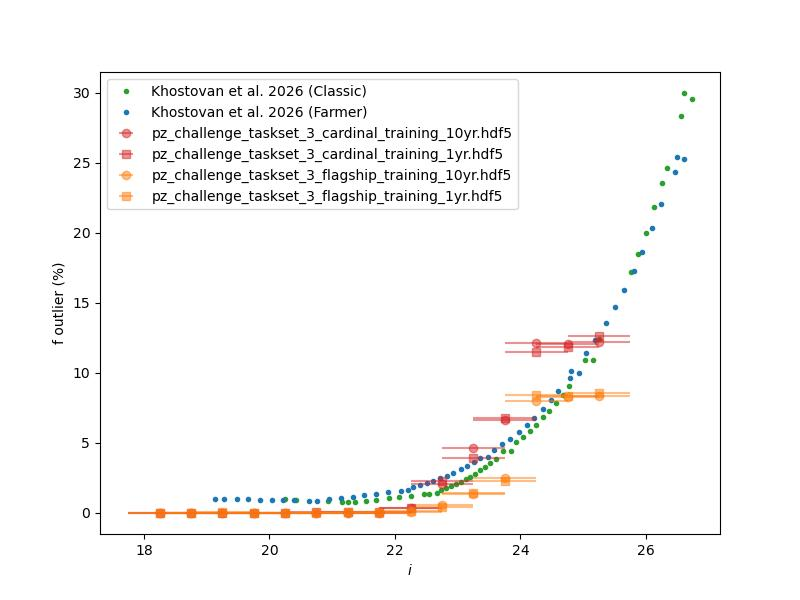
\includegraphics[width=0.45\textwidth]{figures/pz_challenge_taskset_3_training_10yr/foutlier_vs_mag_i}    
    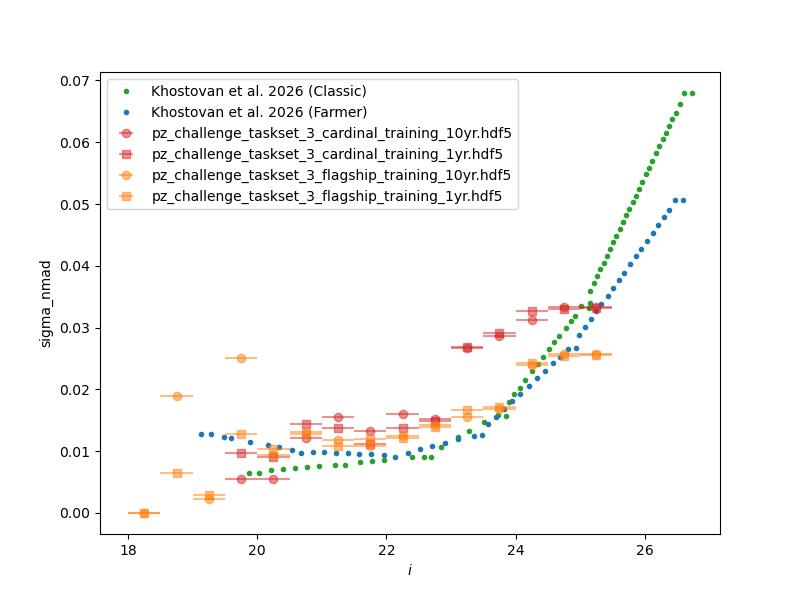
\includegraphics[width=0.45\textwidth]{figures/pz_challenge_taskset_3_training_10yr/sigma_nmad_vs_mag_i}
  }
  \caption{\label{fig:manyband_photoz}\small{Performance of the
      narrow-band photometric redshift estimates as a function of i-band
      magnitude, showing the outlier fraction (left) and width of the
      median absolute deviation (right).}}
\end{figure*}


\subsection{Emulating unrecognized blending}

In the files for taskset 4 we emulate the effect of unrecognized
blending, i.e., two or more objects being detected as a single
object.   Our blending algorithm is relatively simple: we apply a
``friends-of-friends'' matching algorithm with a 1.0 arcsecond linking
length replace all groups with a single object with the summed fluxes
in each of the bands. 


\begin{figure*}[ht]
  \centerline{
    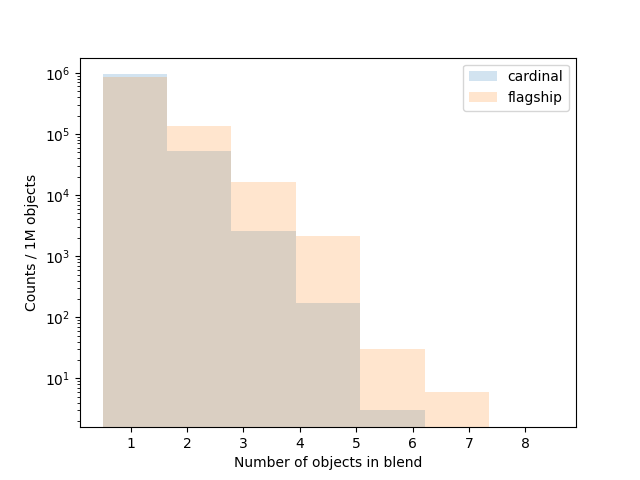
\includegraphics[width=0.45\textwidth]{figures/n_objects_in_blend}    
    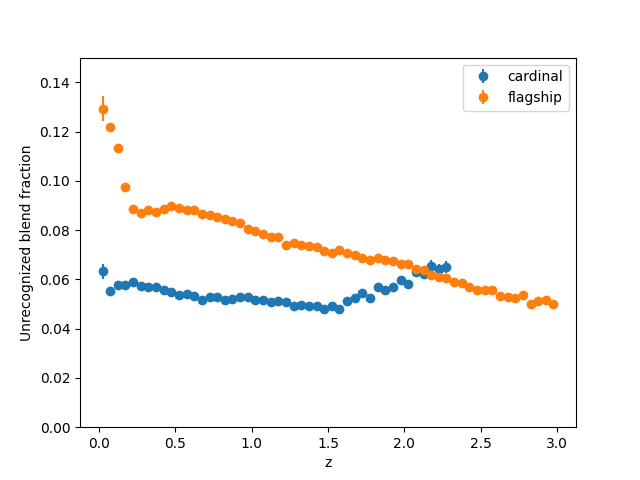
\includegraphics[width=0.45\textwidth]{figures/blend_fractions}
  }
  \centerline{
    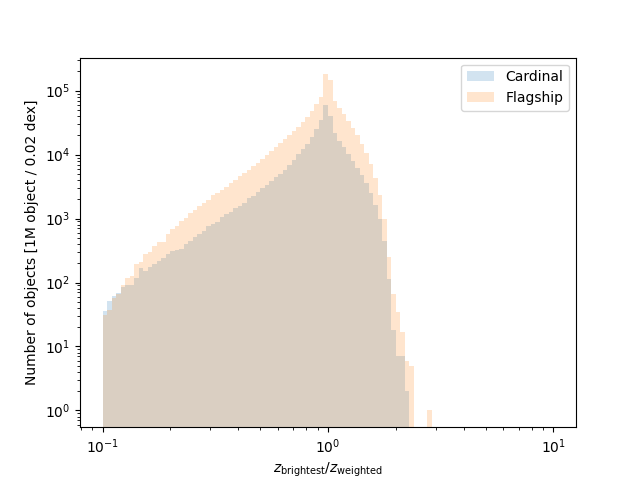
\includegraphics[width=0.45\textwidth]{figures/redshift_ratio}
    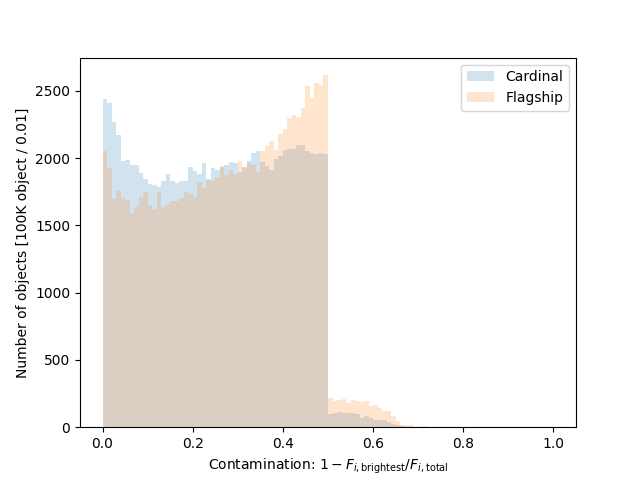
\includegraphics[width=0.45\textwidth]{figures/flux_contamination}
  }
  \caption{\label{fig:blending}\small{Blending behavior.  Top left:
      distribution number of objects in the each blend.  Top right:
      fraction of objects that are blended as a function of redshift.
      Bottom left: ration of the redshift of the brightest object in
      the blend to the flux-weighted mean of all the objects.  Bottom
      right: fraction of the total flux in the blend not from the brightest object.}}      
\end{figure*}



\section{Preparing Training, Test, and Reserved Datasets}
\label{sec:prep_process}

All of the data preparation was performed using the
\texttt{rail\_projects} and \texttt{rail\_package\_config} packages
for bookkeeping and reproducibility.  The scripts listed in Tab.~\ref{tab:prep_scripts}
comprise the entire production pipeline from the simulation truth catalogs
to the files released with the challenge. 

\begin{table}[ht]
\centering
\caption{\label{tab:prep_scripts}\small Scripts used
  in data preparation.}
\begin{tabular}{lll}
\hline \hline
Script & Command Run & Purpose \\ \hline
  do\_00\_reduce & rail-project reduce & Reduce input truth catalogs \\
  &  & (mag. cut and drop columns) \\ 
do\_01\_build & rail-project build & Build configurations to run \\
  &  & truth-to-observed pipeline \\
do\_02\_t2o & rail-project run truth-to-observed & Run truth-to-observed \\
  &  & pipelines to make degraded catalogs \\ 
do\_03\_merge & rail-project merge & Combine spectroscopic selections \\
do\_04\_subselect & rail-project subsample & Make train/test files from catalogs\\
\hline\hline
\end{tabular}
\end{table}


\newpage

\bibliography{pz_challenge.bib}

\end{document}


%  LocalWords:  maketitle fig:pz_redshift_basics includegraphics hdf5
%  LocalWords:  textwidth texttt taskset eac hline hline _lsst pz qp
%  LocalWords:  color_color_redshift_taskset_1_cardinal_10yr github
%  LocalWords:  color_color_redshift_taskset_1_flagship_10yr _1yr.pkl
%  LocalWords:  therailteam2025 iqr schmidt_evaluation_2020 textbf nb
%  LocalWords:  Kullback-Leibler gigaparsecs _subselect newpage zmode
%  LocalWords:  coadded slitless allowbreak _lsst table-io tables_io
%  LocalWords:  texorpdfstring _submission.py _subselect
%  LocalWords:  desicollaboration2025datarelease1dark
